\section{Research Plan}

We expect that the convergent presence of TTX is likely to be related to concurrent gene content, and divide our research project into three stages to leverage from comparison strategies of transcriptomic data across different taxa. Below, we provide details on the material and methods that we will apply at each stage.

\subsection{General research program}

First, we employ RNA-Seq to compare the transcriptomes of different newts from two populations. While in one population the levels of TTX are neglectable, the other population is extremely toxic. Second, deferentially expressed transcripts in both populations are identified, generating a broad list of candidate genes which we will compare with published transcriptomic data of TTX-possessing pufferfishes. On this second stage, we will select transcripts occurring in pufferfish (public data), newts, and frogs (original sequences), if any. Finally, we will try to annotate each transcript select this way with a focus on unknown genes or genes from other TTX-possessing eukaryotes.

\subsection{Hypotheses and objectives}

Our primary objective is the identification of genes involved in TTX chemical defense in the North American salamander \textit{Taricha granulosa}.

If TTX biosynthesis does not involve symbiotic flora in amphibians but is instead the result of concurrent genome content, we should be able to identify genes related to the synthesis of TTX in the genomes of rough-skinned newt by comparing it to the transcriptomes of divergent TTX-possessing taxa.

\subsection{Methods}

This section describes the methods we used to produce our preliminary results. These same methods will be applied to generate new data once our proposal is approved.

\subsubsection{Biological sampling}

For our preliminary analysis, male newts were collected by hand from two locations in the USA: a population from low elevation at Soap Creek Pond (Corvallis, OR), with high amounts of TTX, and another from high elevations on Scotts Lake (a.k.a. ``Lake in the Woods'', Roseburg, OR) with no or very little TTX. Sampling was done in May 2015 by Brodie. We transported the animals to Utah State University where they were housed separately in plastic containers with 2 L of filtered tap water in an environmental chamber at 6 \celsius. We extracted glandular secretions from the animals with the use of a bipolar stimulating electrode (Astro-med, Inc.) to induce the skin glands to secrete their toxins (a procedure often called ``milking'').

We took tissue samples from two males of each of the two populations immediately after collection and forty days after milking. Each sampling provided three skin discs with 5 mm in diameter that we removed using a human skin-biopsy punch. We selected duplicated skin punches that we immersed in RNAlater (Sigma-Aldrich, Catalog Number R0901) for storage at -20 \celsius. Our collaborator, Dr. Ralph A. Saporito (John Carroll University), processed the remaining skin punches for TTX estimation using a Competitive Inhibition Enzymatic Immunoassay \citep[CIEIA; see][]{stokes2012improved}.

We reserved all RNA manipulation into a single clean room. All instruments and bench surface received RNase decontamination solution (RNAse Zap, Life Technologies). We performed RNA fixation from samples of at least 25 mg of tissue per individual.  We only used sterilized razor blades rinsed in RNAse-Zap (Life Technologies). All cleaning procedures were operated as quickly as possible to avoid RNA degeneration in an RNAase-free and cold.

Once this project is approved, we will select five additional individuals from each population for complementary RNA-Seq and transcriptome comparison using the methods described here.

\subsubsection{Total RNA extraction}

We performed total RNA extraction from samples of at least 25 mg of tissue using the TRI Reagent Protocol (Sigma-Aldrich; Catalog no. T9424) following the manufacturer’s protocol. We measured the absorbance of extracted RNA at different wavelengths using a NanoDrop ND-1000 UV spectrophotometer (Thermo Fisher Scientific) to check for contaminants. We also assessed the quantity and purity of mRNA with the fluorometric quantitation performed by the QubiT Fluorometer (Life Technologies). Capillary electrophoresis in an RNA Pico 6000 chip can be implemented using an Agilent Bioanalyzer 2100 System with the ``mRNA pico Series II'' assay (Agilent Technologies, California, USA). For evaluation of the integrity of mRNA, we employed electropherogram profile and checked for the lack of rRNA contamination based on rRNA peaks for 18S and 28S rRNA given by the Bioanalyzer software.

\subsubsection{Library preparation and sequencing}

We shipped RNA eluted in a buffer solution in dry ice (-70 \celsius) to Macrogen (Korea) to perform library preparation and sequencing. At Macrogen’s laboratories, total RNA integrity was checked using an Agilent Technologies 2100 Bioanalyzer(or 2200 TapeStation) with an RNA Integrity Number (RIN) value greater than or equal to 8. Library preparation used TrueSeq Stranded Total RNA LT Sample Preparation (Gold) kit following the TrueSeq Stranded Total RNA Sample Preparation Guide (Part \# 15031048 Rev. E). Macrogen sequenced 4 libraries per lane using an Illumina HiqSeq 2500 with a high throughput mode for paired-end reads of 125 bp each.

The Laboratório de Anfíbios is currently on the process of negotiating to sequence the transcriptome of additional samples at Source Biosciences (UK) using the Illumina TruSeq Stranded Total RNA with RiboZero Gold and the Illumina HiSeq 4000 with 2 x 150 bp paired-end reads.

\subsubsection{Quality control for raw sequence reads}

Quality control was performed by Trimmomatic v0.32 \citep{bolger2014trimmomatic} to remove technical sequences (adapters and primers), low-quality parts of the sequences with an average-quality below 15, individual bases from beginning and end of the sequences with quality less than 3 and reads with less than 36 bases in length.

\subsubsection{Transcriptome assembly}

\textit{De novo} assembly of filtered RNA-Seq reads was executed by Trinity v2.1.1 \citep{grabherr2011trinity}, according to the protocol provided by \citep{haas2013novo}. At first, we assembled libraries individually. After that, the quality of individual assemblies was estimated roughly against a known single-copy orthologs of vertebrates by the software BUSCO v1.1b1 \citep{simao2015busco}. Finally, all samples were pooled and assembled to generate the reference transcriptome. We repeated the same procedure to evaluate the overall quality of the combined assembly.

\subsubsection{Differential expression analysis}

We calculated transcript abundance and estimated expression levels of each transcript reconstructed in the previous step using the RSEM software \citep{li2011rsem}, bidden by Trinity scripts. The procedure has multiple steps. First, aligned reads from individual biological replicate against the transcriptome. After that, we used the number of alignments to each transcript as a proxy to transcript abundance in the samples. Finally, we call upon Bowtie \citep{langmead2009ultrafast} through RSEM software to perform the final re-alignment.

Differently expressed genes were identified by comparing libraries two-by-two, with conservative methods that reduce false-positive results, while allowing false-negatives. Before comparisons, we applied a normalization to accounts for library-specific characteristics. Each library had a different overall number of reads, dependent on methodological artifacts, rather than actual transcript abundance. Moreover, higher read counts could emerge from several transcripts or a few highly expressed ones. Thus, we used the Trimmed Mean of M-values (TMM) normalization method, implemented in the edgeR Bioconductor package \citep{robinson2010edger} with scripts in Trinity, to normalize the read counts among the libraries.

Pairwise comparison among libraries was performed in edgeR, with more scripts in Trinity, to obtain transcript-specific fold changes and \textit{p}-values. For further analysis, we selected only the transcripts with at least 4-fold change and a \textit{p}-value of at most 0.001 in any pairwise comparison. Selected transcripts were clustered in dendrograms and grouped according to 60\% height of the dendrogram.

\subsubsection{Additional sources of RNA data}

\begin{wrapfigure}[13]{L}{0.5\textwidth}
    \centering
    \vspace{-\intextsep}\hspace*{-.75\columnsep}
    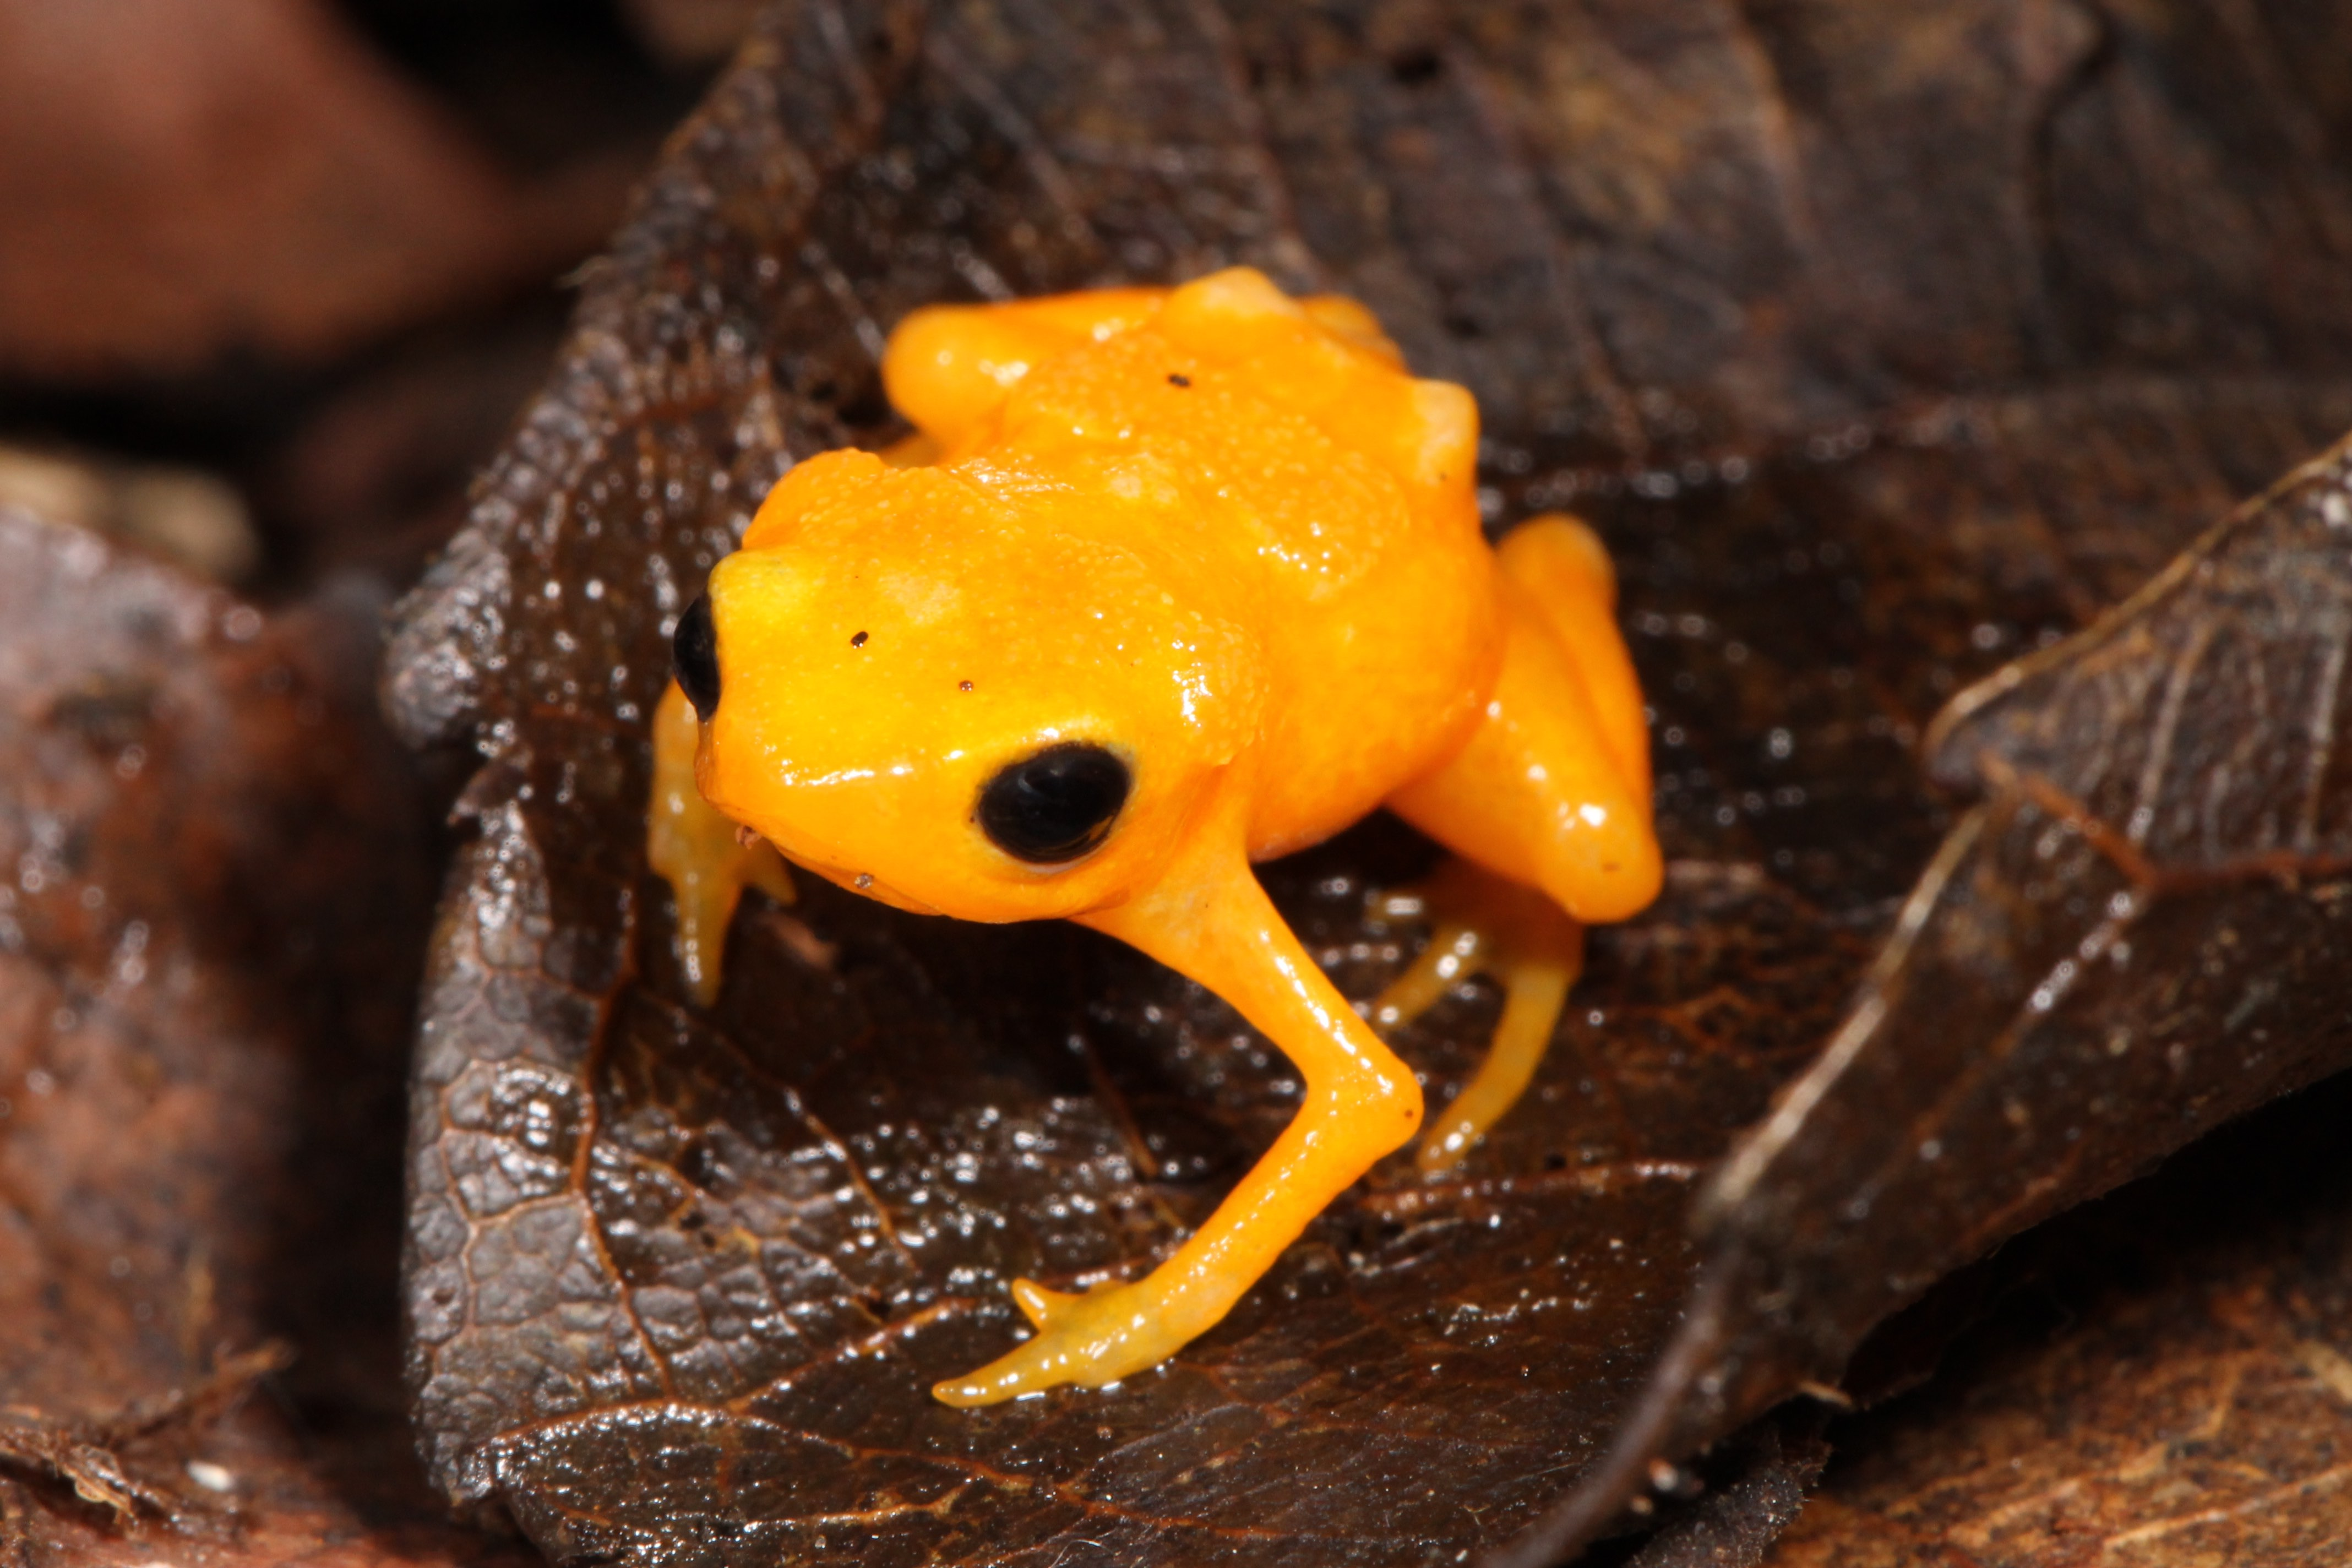
\includegraphics[width=0.48\textwidth]{figs/brachy.jpg}
    \caption{The pumpkin toadlet, \textit{Brachycephalus ephippium}. Credit: Taran Grant.}
    \label{fig:brachy}
\end{wrapfigure}

Original RNA data from frogs of the genus \textit{Brachycephalus} will also be available for this project. Frogs of this genus inhabit the Atlantic Forest and re mostly diminutive, brightly colored, and putatively aposematic. Several publications have reported to have found TTX \citep{sebben1986tetrodotoxin, pires2002occurrence, pires2005further} in \textit{Brachycephalus}. In collaboration with Dr. Brodie’s lab and using a TTX-specific monoclonal antibody for identification and quantification (Stokes et al. 2012), our lab has begun accumulating and analyzing samples from multiple species, populations, and individuals in order to better understand the evolution of TTX-based chemical defense in this clade. In addition to beginning to document variation in TTX-possessing species of \textit{Brachycephalus}, we have confirmed that the cryptically colored species \textit{B. hermogenesi} lacks detectable amounts of TTX while the brightly colored pumpkin toadlet, \textit{Brachycephalus ephippium} (Figure~\ref{fig:brachy}),  is very toxic. As with Taricha granulosa, the Laboratório de Anfíbios has begun analyzing the transcriptome of the pumpkin toadlet in search of genes related to TTX.

Furthermore, this project is counting on public RNA data from other TTX-possing animals, including gastropods and pufferfish \citep[e.g.,][]{aparicio2002whole, gao2014draft, kudo2014draft, jaillon2004genome}.

\subsubsection{Computational resources}

We count on ``ACE'', an SGI rackable computer cluster housed in the Museum of Zoology of the University of São Paulo, for most \textit{in silico} procedures. Selected servers had four 2.3 GHz Operon CPUs with 16 cores each and 256 or 516 GB of memory. After optimization, we were able to reconstruct genomes using a single core and ca. 20 GB of memory. The software environment in ACE consists of a SUSE Linux Enterprise Server with SGI Performance Suite, SGI Management Center and PBS Pro Job Scheduler. For additional details on the computational resources of the Laboratório de Anfíbios, see \href{http://www.ib.usp.br/grant/anfibios/researchHPC.html}{http://www.ib.usp.br/grant/anfibios/researchHPC.html}.

We also count on computational resources from the University of North Carolina at Charlotte, including the computer cluster ``Steelhead'', which comprises five high-memory machines (Dell R815 - 64 AMD cores per node, 512–768 GB RAM each) and a separate computer cluster with 25 nodes, each with 16 CPUs.

\subsubsection{Data management plan}

We will deposit all specimens and associated field notes at the Museu de Zoologia da USP, the Banco de Tecidos de Vertebrados do Departamento de Zoologia da USP or the collections of the Utah State University. For digital data storage, we count on one 64Tb RAID 5.0 server. We may also store digital data on the USP cloud. All data from published studies will be made publicly available either as online supplementary material or through data repositories like NCBI's GenBank (\href{https://www.ncbi.nlm.nih.gov/genbank/}{https://www.ncbi.nlm.nih.gov/genbank/}) and Sequence Read Archive (\href{https://www.ncbi.nlm.nih.gov/sra}{https://www.ncbi.nlm.nih.gov/sra}).